\documentclass[11pt]{article}

\usepackage[margin=0.82in]{geometry}
\usepackage{amsmath,amssymb}
\usepackage{booktabs}
\usepackage{graphicx}
\usepackage{tabularx}
\usepackage{xcolor}
\usepackage{microtype}
\usepackage[hidelinks]{hyperref}

\hypersetup{
  pdftitle={Prism--Eta2 in Plain Language},
  pdfauthor={Prism BA Research Project}
}
\graphicspath{{figures/convergence/}{figures/explanatory/}}
\setlength{\parindent}{0pt}
\setlength{\parskip}{0.68em}
\renewcommand{\arraystretch}{1.16}
\newcolumntype{Y}{>{\raggedright\arraybackslash}X}

\definecolor{deepblue}{HTML}{205B84}
\definecolor{pale}{HTML}{F1F7FA}
\definecolor{warm}{HTML}{FFF6E5}
\definecolor{greenbox}{HTML}{EEF8F2}
\newcommand{\plainbox}[2]{%
  \begin{center}%
  \fcolorbox{#1}{#1!7}{\parbox{0.92\linewidth}{#2}}%
  \end{center}%
}

\title{\vspace{-1.4em}\textbf{Prism--Eta2 in Plain Language}\\[0.35em]
\large What bundle adjustment solves, how curvature is measured, and what the results mean}
\author{Prism BA Research Project\\\small Explanatory companion to the technical report}
\date{13 September 2026}

\begin{document}
\maketitle

\begin{abstract}
Bundle adjustment adjusts camera parameters and 3D points so that the points project onto their measured image locations.  Prism--Eta2 solves this problem on a GPU by eliminating the point variables, approximately solving the remaining camera system, and checking every proposed update against the real image error.  This report explains that process without assuming expertise in numerical optimization.  Particular attention is given to the word \emph{curvature}.  In Eta2, the active curvature guard does not estimate the curvature of the true nonlinear bundle-adjustment objective.  It measures the bending of the current \emph{numerical damped quadratic model} along one PCG search direction.  The exact measured quantity is $q=(p^TAp)/(p^Tp)$, obtained from data PCG already computes.  A separate quantity, $\rho$, later checks whether the completed camera--point proposal actually behaved like the nonlinear model predicted.  Keeping these two tests separate is essential for understanding both the method and its novelty.
\end{abstract}

\plainbox{deepblue}{\textbf{The short version.}
Eta2 repeatedly builds a local quadratic approximation of the image error, solves it only approximately, limits the camera motion, recovers the point motion, and then evaluates the real image error.  During the approximate camera solve, it checks whether the numerical quadratic bends upward along the current PCG direction.  If the measured bending is zero or negative, it increases damping, rebuilds the affected linear system, and starts PCG again.  This is a safety repair.  It does not accept a camera update, and it was inactive in the practical-target runs that produced the headline speed results.}

\tableofcontents

\section{What problem are we solving?}

Imagine that we have many photographs of the same scene.  Each photograph comes with an approximate camera pose and camera calibration, and each visible feature has an approximate 3D location.  If the estimates were perfect, projecting every 3D point through every camera would land exactly on the measured image feature.  Usually it does not.

For an observation of point $j$ in camera $i$, let
\[
  r_{ij}=\hbox{predicted pixel location}-\hbox{measured pixel location}.
\]
This is a two-number vector: horizontal and vertical pixel error.  Bundle adjustment changes all camera parameters $c_i$ and point locations $X_j$ to minimize
\begin{equation}
  F(c,X)=\frac12\sum_{(i,j)\in\mathcal O}\lVert r_{ij}(c_i,X_j)\rVert^2. \label{eq:plain-objective}
\end{equation}
Lower is better.  The factor $1/2$ only makes derivatives cleaner.

The experiments in this project always score the same objective: the same original observations, the SIMPLE\_RADIAL camera model, one active radial-distortion coefficient, unshared intrinsics, and the second radial coefficient fixed to zero.  There is no hidden robust loss or deleted-observation advantage in the reported score.

\subsection{Why this is difficult}

Three properties make large bundle adjustment challenging:

\begin{enumerate}
  \item \textbf{Scale.}  Final-13682 has 13,682 cameras, 4,456,117 points, and 28,987,644 observations.
  \item \textbf{Coupling.}  Moving a camera changes every point seen by it; moving a point affects every camera that sees it.
  \item \textbf{Nonlinearity.}  Perspective projection divides by depth.  Near zero depth, a tiny state change can cause a very large pixel change.  A quadratic approximation is trustworthy only locally.
\end{enumerate}

\section{What one Eta2 iteration does}

An outer iteration follows this sequence:

\begin{center}
\fbox{linearize pixel errors}
$\longrightarrow$
\fbox{eliminate points}
$\longrightarrow$
\fbox{approximately solve cameras}
\\[0.8em]
$\longrightarrow$
\fbox{limit camera step}
$\longrightarrow$
\fbox{recover point step}
$\longrightarrow$
\fbox{measure real cost}
\\[0.8em]
$\longrightarrow$
\fbox{accept, reject, or try a safe repair}
\end{center}

``Linearize'' means replacing the curved residual function near the current state by a straight-line approximation,
\[
  r(x+d)\approx r(x)+Jd,
\]
where $J$ is the Jacobian and $d$ is the proposed state change.  Squaring this approximation produces a quadratic model.  Levenberg--Marquardt (LM) adds positive damping so that poorly observed directions do not move too far.

Splitting camera and point variables gives the block system
\begin{equation}
\begin{bmatrix}
U+\lambda D_c & W\\
W^T & V+\lambda D_p
\end{bmatrix}
\begin{bmatrix}d_c\\d_p\end{bmatrix}
=-
\begin{bmatrix}g_c\\g_p\end{bmatrix}. \label{eq:plain-normal}
\end{equation}
Here $U$ describes camera-only effects, $V$ point-only effects, and $W$ camera--point coupling.  The scalar $\lambda$ is the damping level.  Eta2 couples camera and point damping to the same $\lambda$.

\section{Why the solver eliminates points}

Every 3D point has only three unknown coordinates, and observations do not directly connect one point to another.  Therefore $V+\lambda D_p$ consists of independent $3\times3$ point blocks.  Those small blocks are cheap to solve.  Eliminating them gives a camera-only system
\begin{equation}
  A_\lambda z=b_\lambda, \label{eq:plain-schur}
\end{equation}
where $z$ is a diagonally scaled camera update and
\begin{equation}
  A_\lambda
  =E\left(U-W(V+\lambda D_p)^{-1}W^T\right)E+\lambda I. \label{eq:plain-A}
\end{equation}
This is the damped, scaled Schur complement.

Prism does not store the huge matrix $A_\lambda$.  When PCG asks for $A_\lambda p$, GPU kernels traverse the observations, perform the small point solves, and accumulate the answer for each camera.  This is what \emph{matrix-free Schur} means here: the mathematical matrix exists, but the code evaluates its action on a vector instead of materializing all its entries.

After finding the camera update $d_c=Ez$, the point update is recovered by
\begin{equation}
  d_p=-(V+\lambda D_p)^{-1}(g_p+W^Td_c). \label{eq:plain-backsub}
\end{equation}

\section{What ``Eta2'' means}

PCG could solve Eq.~\eqref{eq:plain-schur} to very high accuracy.  Eta2 usually chooses not to.  The reason is practical: a very accurate answer to an imperfect local quadratic model can cost more and can move into nonlinear directions that the model does not describe well.

The solver computes a requested relative residual tolerance $\eta$.  Its baseline rule uses the change in reduced right-hand-side norm, then Eta2 multiplies that tolerance by two and caps it at 0.5:
\[
  \eta=\operatorname{clip}_{[10^{-12},0.5]}
  \left(2\min\left[0.5,0.9\left(\frac{\lVert b_k\rVert}{\lVert b_{\rm prev}\rVert}\right)^2\right]\right).
\]

\plainbox{deepblue}{\textbf{Common misunderstanding:} ``Eta2'' does not mean $\eta=2$.  It means ``twice the baseline adaptive tolerance,'' with a maximum of 0.5.  A larger tolerance permits an earlier, cheaper PCG stop.}

Because PCG stops early, its particular finite iterate matters.  Changing the preconditioner, arithmetic, or operator can return another direction that satisfies the same residual tolerance but sends the nonlinear solver into a different future trajectory.

\section{Curvature: the exact quantity Eta2 measures}\label{sec:curvature}

This is the central clarification.

During PCG, let $p$ be the current search direction in the scaled camera coordinates.  PCG already computes
\[
  A_\lambda p
\]
to update its residual.  Eta2 takes two dot products:
\begin{align}
  pAp &= p^T(A_\lambda p),\\
  pp  &= p^Tp,
\end{align}
and defines the normalized directional curvature
\begin{equation}
  q=\frac{p^TA_\lambda p}{p^Tp}. \label{eq:rayleigh}
\end{equation}
This is a Rayleigh quotient.  It answers one narrow question:

\begin{quote}
\emph{Along this particular PCG direction, does the current numerical damped quadratic model bend upward, remain nearly flat, or bend downward?}
\end{quote}

To see why, restrict a quadratic model $m$ to steps of the form $z+\alpha p$:
\begin{equation}
  m(z+\alpha p)=m(z)+\alpha\nabla m(z)^Tp
    +\frac12\alpha^2 p^TA_\lambda p. \label{eq:linequad}
\end{equation}
The coefficient $p^TA_\lambda p$ controls the bending along the line.  Division by $p^Tp$ expresses that bending per unit squared direction length.

\begin{figure}[ht]
\centering
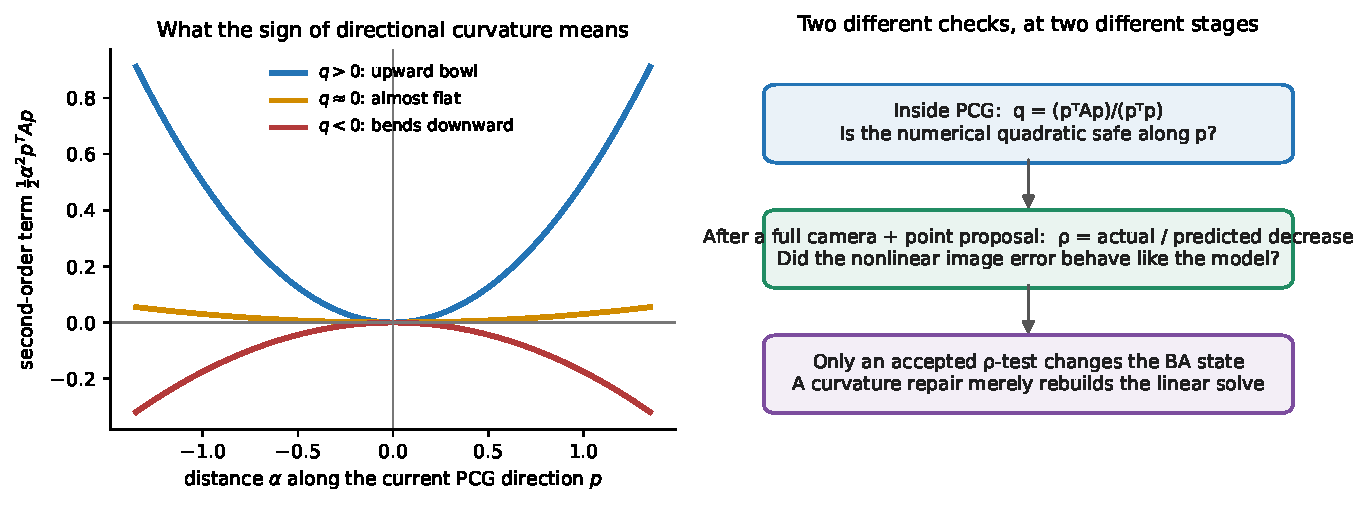
\includegraphics[width=\textwidth]{directional_curvature.pdf}
\caption{Left: the sign of $p^TAp$ controls the second-order bending along one direction.  Right: the PCG curvature test $q$ and the later nonlinear gain-ratio test $\rho$ answer different questions.  This figure is schematic; it is not a plot of a BAL trajectory.}
\label{fig:curvature}
\end{figure}

The actual check in the frozen source is equivalent to:
\begin{verbatim}
Ap  = ApplyDampedSchur(p)
pAp = dot(p, Ap)
pp  = dot(p, p)
q   = pAp / pp

if not (pAp > 1e-14 * pp):
    trigger numerical-curvature recovery
else:
    continue the ordinary PCG recurrence
\end{verbatim}
Thus the check has almost no extra algebraic cost: $A_\lambda p$ and $p^TA_\lambda p$ are already needed for the ordinary PCG step length.

\subsection{How to interpret the sign}

\begin{itemize}
  \item $q>0$: the quadratic bends upward along $p$, as expected for a safely damped Gauss--Newton model.
  \item $q\approx0$: the model is nearly flat along $p$.  Dividing by $p^TAp$ in the CG step can produce a very large or numerically unstable move.
  \item $q<0$: the numerical quadratic bends downward along $p$.  Ordinary positive-definite CG assumptions do not hold for that direction.
\end{itemize}

The guard uses the scale-aware condition $p^TAp>10^{-14}p^Tp$, rather than testing $p^TAp>0$ exactly.  The camera coordinates have already been normalized by the camera diagonal scaling $E$, which makes the threshold more meaningful across parameters with very different physical units.

\subsection{What this measurement is not}

The curvature $q$ is \textbf{not}:

\begin{itemize}
  \item an eigenvalue calculation of the whole Schur matrix;
  \item the curvature of the 3D camera path or reconstructed surface;
  \item the second derivative of the full nonlinear pixel objective;
  \item a finite-difference evaluation of $F(x+hp)$;
  \item the omitted residual-Hessian term $\sum_k r_k\nabla^2r_k$;
  \item the gain ratio $\rho$ used to accept a completed nonlinear step; or
  \item a learned curvature feature or RL action.
\end{itemize}

A negative sampled quotient proves that the implemented numerical operator is unsafe along that sampled direction.  Positive quotients for all directions visited by PCG do not prove that every possible direction is positive.

\section{Why can a damped Gauss--Newton curvature become negative?}

If all blocks were formed exactly from one Jacobian, $J^TJ$ would be positive semidefinite, and positive damping would make the active system positive definite.  The implementation is more complicated: compact camera--point fragments are stored in FP32, while camera blocks, point factorization, accumulation, and PCG use substantial FP64 arithmetic.  The separately rounded $U$, $W$, and $V$ therefore need not equal the three blocks of one exact stored Jacobian.

The Schur term subtracts two quantities,
\[
  U-W(V+\lambda D_p)^{-1}W^T.
\]
When those quantities nearly cancel, a small mismatch can change the sign of the remaining tiny number.  Poorly conditioned two-observation tracks make the problem worse because the inverse point block amplifies small cross-block errors.  This is like subtracting $1.0000001$ from $1.0000000$ after the two values have been rounded differently: the small answer is governed by the rounding, not by the accuracy of either large term alone.

This diagnosis is measured, not only hypothetical:

\begin{table}[ht]
\centering
\small
\caption{Two captured Ladybug directions.  Reconstructing a coherent Schur energy from original FP64 Jacobians changes the sign while holding the state, direction, and damping fixed.}
\begin{tabular}{@{}lrrr@{}}
\toprule
Captured outer & Stored $p^TAp$ & Coherent FP64 Schur energy & Point-solve rel. residual\\
\midrule
15 & $-71.971990$ & $273.672298$ & 0.134\\
16 & $-10.225014$ & $40.295156$ & 0.712\\
\bottomrule
\end{tabular}
\end{table}

In a second same-state audit on three Venice captures, FP32 cross blocks produced normalized quotients from approximately $-0.56\times10^{-9}$ to $-2.57\times10^{-9}$.  Changing only those cross blocks to FP64 made them positive, approximately $3.43\times10^{-8}$ to $4.28\times10^{-8}$.  Rebuilding only the point factor did not fix them.  Two ill-conditioned, two-observation tracks dominated the discrepancy.

This does not mean every late Venice state has a negative numerical operator.  Eighteen independently supplied states were positive under their registered damping.  The failure is trajectory- and state-dependent.

\section{What happens after the curvature check fires?}

Suppose Eq.~\eqref{eq:rayleigh} gives $q$ at damping $\lambda$.  The frozen recovery chooses
\begin{equation}
  \lambda'=4\max(\lambda,\lambda-q), \label{eq:plain-repair}
\end{equation}
clipped to the implementation's range $[10^{-14},10^{16}]$.  It then:

\begin{enumerate}
  \item raises a persistent numerical damping floor;
  \item rebuilds the damped $3\times3$ point factors;
  \item rebuilds the reduced right-hand side and camera preconditioner;
  \item discards the old PCG recurrence, because it belongs to another operator; and
  \item starts PCG again at the same nonlinear state.
\end{enumerate}

The state of the cameras and points has not changed.  The solver has only replaced an unsafe local linear problem by a more strongly damped one.

\subsection{A numerical example}

Take $\lambda=10^{-10}$ and suppose PCG measures $q=-2\times10^{-8}$.  Then
\[
  \lambda'=4(10^{-10}+2\times10^{-8})=8.04\times10^{-8}.
\]
For frozen blocks, increasing the coupled damping from $\lambda$ to $\lambda'$ increases the Rayleigh quotient of the same direction by at least $\lambda'-\lambda$.  Therefore
\[
  q(\lambda')\ge -2\times10^{-8}+(8.04\times10^{-8}-10^{-10})
  =6.03\times10^{-8}>0.
\]
This is a directional guarantee in exact arithmetic.  It is not a guarantee that every direction of the rebuilt numerical operator is positive, so the next PCG run still checks its own directions.

\plainbox{greenbox}{\textbf{Why the floor persists.}  If the controller immediately returned to the tiny damping that exposed the numerical failure, it could repeat the same breakdown.  Retaining the repaired value as a lower bound prevents that immediate loop.  The floor can over-damp later work, so it is a bounded safeguard rather than a free acceleration.}

\section{\texorpdfstring{Curvature $q$ versus gain ratio $\rho$}{Curvature q versus gain ratio rho}}

These quantities are often confused because both relate to the local model.

\begin{table}[ht]
\centering
\small
\caption{The curvature guard and nonlinear acceptance test occur at different stages.}
\begin{tabularx}{\textwidth}{@{}lYY@{}}
\toprule
 & Directional curvature $q$ & Gain ratio $\rho$\\
\midrule
When measured & Inside every PCG iteration & After a complete camera--point candidate exists\\
Formula & $(p^TA_\lambda p)/(p^Tp)$ & actual objective decrease / predicted decrease\\
Uses true new image cost? & No & Yes\\
Question & Is the numerical quadratic safe along this PCG direction? & Did the nonlinear objective behave like the model?\\
Failure response & Increase damping, rebuild, restart PCG & Reject or contract the radius/damping controller\\
Changes BA state? & No & Only if the candidate passes acceptance\\
Frozen thresholds & unsafe if $q\le10^{-14}$ & accept only with $\rho>0.1$ plus descent and radius checks\\
\bottomrule
\end{tabularx}
\end{table}

For a completed candidate $d$, Eta2 directly evaluates
\begin{align}
  \operatorname{pred}(d)&=-g^Td-\frac12\lVert Jd\rVert^2,\\
  \rho&=\frac{F(x)-F(x\oplus d)}{\operatorname{pred}(d)}.
\end{align}
The prediction is recomputed on the actual step after camera clipping and point safeguards.  A direction can have perfectly positive $q$ and still have poor $\rho$: the quadratic may be numerically valid but inaccurate for the nonlinear perspective projection over that step length.  This exact separation was observed in the Venice precision study: FP64 cross blocks removed all ten curvature truncations, yet all ten resulting de-clipped proposals still failed nonlinear acceptance.

\section{Radius limiting and the point safeguard}

PCG returns a scaled camera vector $z$.  Eta2 limits its norm to radius $R$:
\[
  z\leftarrow z\min(1,R/\lVert z\rVert).
\]
It then recomputes the point update using the limited camera step.  This keeps camera motion bounded, but it is not the exact classical trust-region solution and it does not uniformly scale a completed camera--point step.

For an eligible failed proposal, Eta2 can try shorter steps.  It can also hold the proposed cameras fixed and let each point track choose between its old and proposed position.  At fixed cameras the tracks are independent, so
\[
  F(c^+,\widetilde X)=\sum_j\min\{F_j(c^+,X_j),F_j(c^+,X_j+d_j)\}.
\]
This finds the best of all $2^{n_p}$ binary keep/move point combinations with one linear pass over the observations.  It still must beat the old joint state and pass the global model and acceptance checks.

\section{What produced the measured speed?}

The headline practical-target speed should not be credited to the curvature guard.  On the frozen three-instance, nine-target speed panel, numerical recovery activated zero times before the targets.  On Final-13682, Eta2 reached the primary target with zero rejects and zero repairs.

The measured speed comes primarily from:
\begin{itemize}
  \item a single damping candidate rather than a multi-shift menu;
  \item Eta2's deliberately loose PCG forcing rule;
  \item matrix-free GPU Schur products and compact storage;
  \item few accepted outer iterations on the stable target paths; and
  \item later systems work that reduces synchronization and dead preparation work.
\end{itemize}

The curvature recovery is best described as a tail-safety mechanism with a clear numerical interpretation.  It improved observed reliability on specific captured Ladybug paths, but a simpler retained damping floor often matched it.  Its incremental general speed advantage is not established.

\section{Results in simple terms}

\subsection{Largest BAL scene}

The common target acts like a finish line: every solver must lower the exact same pixel-error objective below $27{,}591{,}576.56$.  Time is recorded only when an independently rescored endpoint is on the correct side of that line.

\begin{table}[ht]
\centering
\small
\caption{Final-13682 native time to the same useful-quality target.}
\begin{tabular}{@{}lccc@{}}
\toprule
Solver & Hits & Median seconds & Relative to Eta2\\
\midrule
Prism Eta2 & 5/5 & \textbf{3.239} & $1.00\times$\\
Previous Prism incumbent & 5/5 & 4.262 & $1.32\times$ slower\\
Caspar FP32 & 3/3 & 7.084 & $2.19\times$ slower\\
Caspar FP64 & 3/3 & 14.973 & $4.62\times$ slower\\
\bottomrule
\end{tabular}
\end{table}

Eta2 uses four accepted outer iterations and 19 Schur products, with zero rejects.  At a tighter target, its advantage over the previous Prism configuration shrinks to 1.035$\times$.  The strongest evidence is therefore fast arrival at useful quality, not a uniform advantage at every late-convergence threshold.

\begin{figure}[ht]
\centering
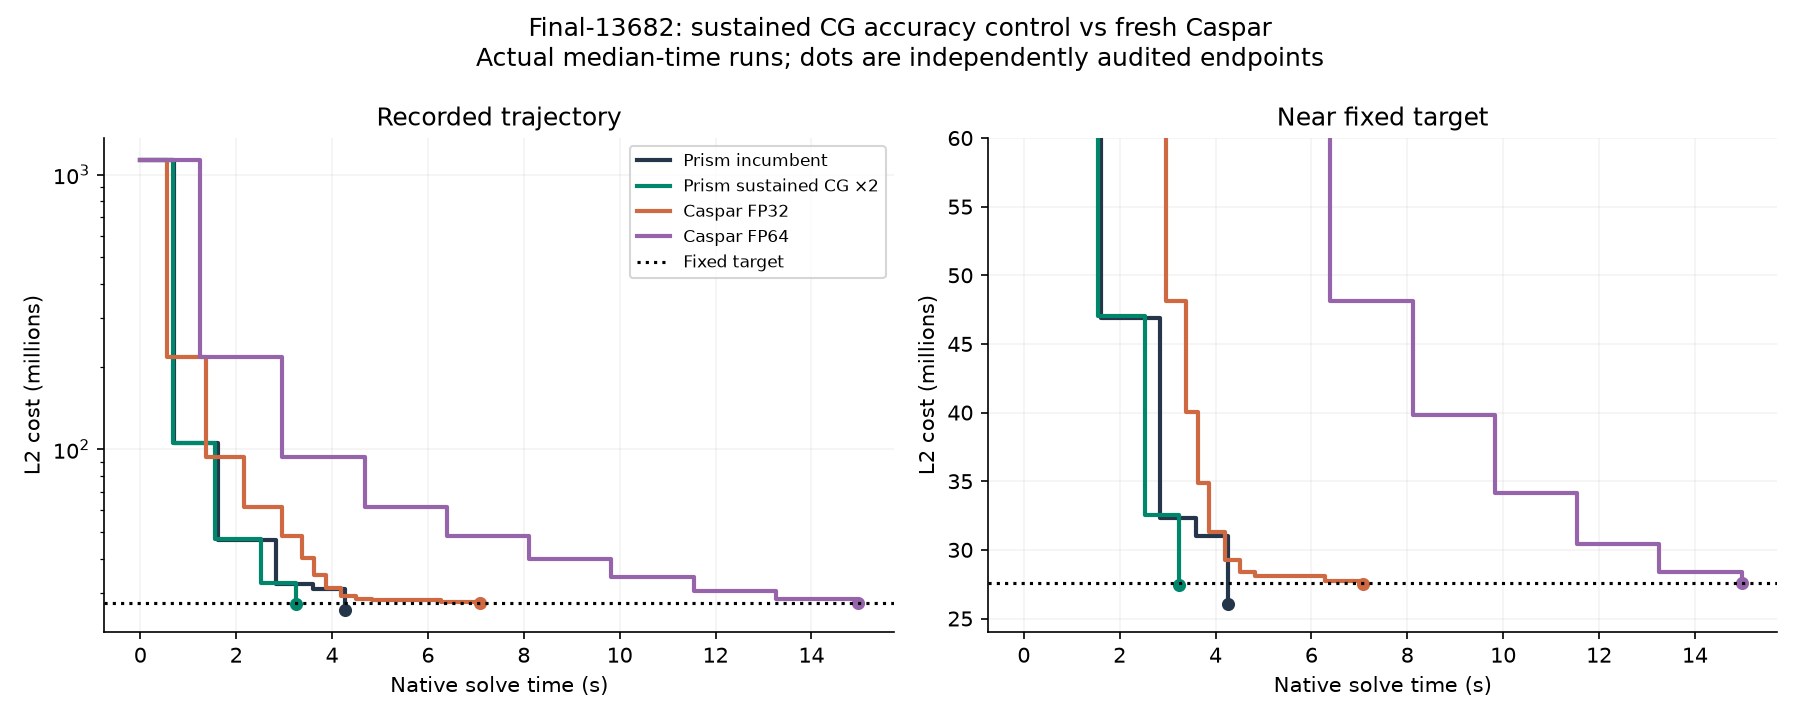
\includegraphics[width=0.98\textwidth]{final13682_sustained_caspar.png}
\caption{Recorded convergence on Final-13682.  Lower objective is better; moving left means reaching that quality sooner.  The horizontal dashed line is the common primary target.}
\label{fig:largest-plain}
\end{figure}

\subsection{Three additional BAL instances}

At the primary target on each scene, median native times were:

\begin{table}[ht]
\centering
\small
\caption{Primary-target seconds, $N=3$.  A miss is left as a miss.}
\resizebox{\textwidth}{!}{%
\begin{tabular}{@{}lccccc@{}}
\toprule
Scene & Eta2 & Caspar FP32 & Caspar FP64 & Ceres LM, CPU & Ceres Dogleg, CPU\\
\midrule
Ladybug-539 & \textbf{0.0808} & 0.1360 & 0.2557 & 1.6517 & 2.9110\\
Trafalgar-138 & \textbf{0.2443} & 0/3 hits & 0/3 hits & 3.0499 & 2.9190\\
Final-394 & \textbf{0.1862} & 1/3 hits & 3.0683 & 4.6668 & 7.4372\\
\bottomrule
\end{tabular}}
\end{table}

Across three registered target tolerances per scene, Eta2 reached 27/27 targets and was fastest among the measured configurations in all nine cells.  Caspar FP32 reached 16/27, Caspar FP64 21/27, and both Ceres CPU arms 27/27.  This supports ``fastest among these tested configurations on this host.''  It does not prove that Eta2 is the fastest possible BA solver or faster than every untested GPU system.

\subsection{The optimized B6v7 implementation}

B6v7 preserves the method but changes GPU execution.  On problems with at least 128 cameras, it uses a camera-owned reduced-RHS reduction, removes dead diagonal preparation, and batches independent FP64 PCG dot returns.  It is 8.66\% faster in geometric-mean time-to-target across the nine practical cells and 4.05\% faster on Muell, with the same stable-cell products, outers, and rejects.

On the variable Final-3068 scene, a 150-run-per-arm study measured 100/150 B6v7 hits versus 89/150 for its control.  Conditional median crossing time improved from 3.669 to 3.269 seconds.  The hit-rate result passed a registered non-inferiority test; statistical superiority was not established.

\section{What is plausibly novel?}

The broad ingredients---LM, Schur elimination, PCG, diagonal damping, inexact forcing, trust ratios, and point inner iterations---are established methods\cite{Agarwal2010,Triggs2000,EisenstatWalker1996,Conn2000,Jeong2012}.  Square-root BA also documents the numerical stability problem of subtractive Schur marginalization\cite{Demmel2021}.

The defensible contribution is narrower:

\begin{enumerate}
  \item an integrated GPU solver that spends little work on the local solve and validates the actual modified nonlinear candidate;
  \item the linear-work, per-track old/full point selection with the exact binary separability guarantee;
  \item a measured mixed-storage Schur failure, a thin-track amplification diagnosis, and persistent coupled damping recovery with a directional bound;
  \item concrete counterexamples showing that a more accurate, better conditioned, or more backward-stable linear solve can produce a worse nonlinear BA trajectory under loose forcing; and
  \item B6v7's separately measured systems path.
\end{enumerate}

The present evidence does not support describing Eta2 as a new general trust-region method.  It also does not support crediting multi-shift CG or RL: both are disabled in the frozen champion.  Priority for the exact point-selection policy and the full numerical-recovery combination still needs an exhaustive literature and patent search before formal publication language is fixed.

\section{Questions a reader is likely to ask}

\textbf{Does negative $q$ mean the true BA objective has a saddle?}

No.  The measured cases were numerical failures of the damped Gauss--Newton Schur operator.  Recomputing coherent FP64 energies changed their signs.  Eta2 does not measure the full nonlinear Hessian.

\textbf{Does positive $q$ mean the step will be accepted?}

No.  Positive $q$ only permits PCG to continue.  The full camera--point candidate can still fail the real-cost or $\rho$ test.

\textbf{Does the curvature repair choose the best damping?}

No.  It chooses a conservative larger damping intended to repair the observed direction.  The ordinary radius and damping controller continues afterward.

\textbf{Is curvature measured with extra finite differences or extra objective evaluations?}

No.  The active guard uses $p$, $A_\lambda p$, and dot products already present in PCG.  Separate research diagnostics did use finite differences, but they are not the frozen guard.

\textbf{Did curvature recovery cause the Final-13682 speedup?}

No.  There were no repairs on that target path.  Eta2's forcing and the efficient single-shift GPU path explain the practical speed result.

\textbf{Why report time-to-target rather than only final error?}

A solver that stops earlier can have a slightly different terminal cost simply because accepted iterations are discrete.  A common target asks the convergence question directly: how long does each method need to achieve the same useful quality?

\section{Evidence and reproducibility}

The frozen configuration is in \path{../champion.json}; source hashes are in \path{../source_manifest.json}.  The main supporting reports are:

\begin{itemize}
  \item \path{theory_and_novelty.md}: full equations and claim boundary;
  \item \path{rl_sustained_results.md}: six-scene selection and Final-13682;
  \item \path{speed_novelty_results.md}: three-instance external-baseline panel;
  \item \path{model_followup_results.md} and \path{schur_recovery_results.md}: captured curvature failures and controls;
  \item \path{../../eta2_pair_precision/FINDINGS.md}: same-state cross-block precision audit; and
  \item \path{../../eta2_wave5/B6V7_RESULTS.md}: optimized systems candidate.
\end{itemize}

\begin{thebibliography}{99}
\small
\bibitem{Agarwal2010}
S. Agarwal, N. Snavely, S. Seitz, and R. Szeliski,
``Bundle Adjustment in the Large,'' ECCV 2010.

\bibitem{Triggs2000}
B. Triggs, P. McLauchlan, R. Hartley, and A. Fitzgibbon,
``Bundle Adjustment---A Modern Synthesis,'' LNCS 1883, 2000.

\bibitem{EisenstatWalker1996}
S. Eisenstat and H. Walker,
``Choosing the Forcing Terms in an Inexact Newton Method,''
SIAM Journal on Scientific Computing 17(1), 1996.

\bibitem{Conn2000}
A. Conn, N. Gould, and P. Toint,
\emph{Trust-Region Methods}, SIAM, 2000.

\bibitem{Jeong2012}
Y. Jeong, D. Nist\'er, D. Steedly, R. Szeliski, and I.-S. Kweon,
``Pushing the Envelope of Modern Methods for Bundle Adjustment,''
IEEE TPAMI 34(8), 2012.

\bibitem{Demmel2021}
N. Demmel, C. Sommer, D. Cremers, and V. Usenko,
``Square Root Bundle Adjustment for Large-Scale Reconstruction,'' CVPR 2021.

\end{thebibliography}

\end{document}
